\section{Versuchsdurchführung}
\label{sec:versuchsdurchfuehrung}

die Versuchsdurchführungen fanden an drei Orten statt
auf dem Balkon in Unterilp in Heiligenhaus
Dachterrasse vom Stundentenwohnheim des Campus Velbert/Heiligenhaus sowie die Dachterrasse vom Campus selbst

insgesamt gibt es 82? h Daten, die das Programm in den Versuchsdurchführung aufgenommen und analysiert hat

Im folgenden ist beschrieben wie die einzelnen Versuche durchgeführt wurden und welche Ergebnisse dabei herauskommen,. Diese sind im Anschluss jeweils validiert. Am Ende gibt es ein Ranking, welche Top fünf Vögel bei einer bestimmten Wahrscheinlichkeit in der Klassifikation (wie umschreibt man confidence?) vorhergesagt wurden.


\subsection{Realer Aufbau}

Bilder vom Versuchsaufbau mit der Hardware -< nur den Inhalte der Horchbox erklären

mobiler Computer liegt in der Horchbux
GPS-Tracker und Mikrofon per USB-Kabel an die USB-Port angeschlossen
Die Kabel sind durch die abgedichteten Löcher des Box durchgeführt, um die Box zu verschließen, aber die kabel nach draußen führen zu können.

Für diesen hier dargstellten Aufgbau sei noch folgende zu wissen.
Mikrofon ist an einem verlängerten USB-Kabel (wie lang?) angeschlossen. Zusätzlich liegt zwischen Verlängerungskabel und Mikrofonklingenanschluss ein Adapter (Klingenanschluss zu USB). Dieses sollte einen möglichst weiten Abstand zu dem hier genutzen Nividia Jetson (Nochmal bibiligraphy auf den Jetson referenzieren?) haben, da es sonst zu Interferenzstörungen kommt.


Zum Start ist der Host-Computer mit dem mobilen Computer per Hotspot vom mobilen Computer verbunden. Die Anwendung bekommt das den cmd-Befehl mit den entsprechenden Starargumenten, wordurch die Audiosession gestartet wird.

(Empfehlung aussprechen es über eine tmux shell zu starten?)

Bei jedem Test unterscheiden sich einige Startargumente zu den vorherigen.



%eine einleitende Tabelle die die erste Spalte (Ordner, Datum etc. erklärt)

Vorbereitende Tests:

testen, wie gut es menschen erkennt
testen, wie gut das Mikrofon aufnehmen kann


\subsubsection{Menschenfilter - Test}

mit einer Wahrscheinlichkeit unter 0.3 Kirchenglocke als Mensch erkannt. Das ist ein Problem, denn bei einem overlap größer 0, wo dann die Zeitintervalle der Vögel und der Kirchenglocke gleichzeitig  zu hören sind, würde das Programm diese Vögel rauswerfen, obwohl das nicht nötig ist.

-> Beispiel in Wohnheim\_Dachterrasse\_100524 um 7 Uhr



\subsection{Testversuch 1: Wohnheim Dachterrasse}

Der erste Testversuch ist in mehreren Testversuche aufgeteilt, um die Analysezeit des Netzes im Multiprocessing zu testen, wenn verschiedene Werte für das Startargumente \texttt{--overlap} zu testen. 
Alle drei Teile des Testversuchs fanden auf der Dachterrasse des Wohnheims statt. Hier der Aufbau:

\begin{figure}
    \centering
    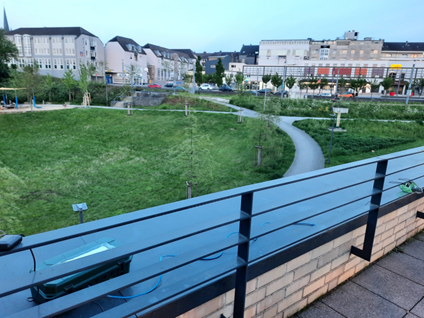
\includegraphics[width=1\linewidth]{bilder/wohnheim_01.png}
    \caption{Bild vom Versuchsaufbau und der Umgebung}
    \label{fig:enter-label}
\end{figure}

\begin{figure}
    \centering
    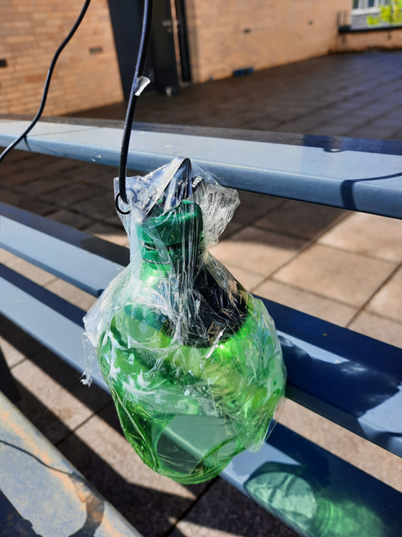
\includegraphics[width=0.5\linewidth]{../grafik.png}
    \caption{Mikrofon in einem Wasserflaschenkopf zum Schutz vor eventuellem Regen}
    \label{fig:enter-label}
\end{figure}

\begin{figure}
    \centering
    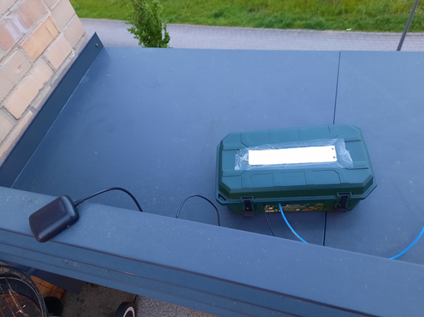
\includegraphics[width=1\linewidth]{../wohnheim_03.png}
    \caption{weiteres Bild vom Versuchsaufbau mit Horchbox und GPS-Tracker}
    \label{fig:enter-label}
\end{figure}

Insgesamt hat dieser ...(26h?) gedauert.
Die einzelnen Testversuche haben ...(12?) Stunden, vier Stunden und zehn Stunden gedauert.

%kurze 

\subsubsection{Testversuch 1.1}

Einstellungen:

Auflistung oder Text oder Bild?

Eckdaten:

Datum: 10.~05.~24
Dauer: 12 h
Ordner: COUNTRIES/Deutschland/Heiligenhaus/Wohnheim\_Dachterrasse\_100524
Koordinaten vom GPS: ja




Da das GPS-Gerät nicht den richtigen Tag bestimmen konnte, liegt das Datumsstempel für die Dateinamen um zwei Tag zurück. Jedoch stimmen die Uhrzeiten, weswegen es für die Validierung der Testergebnisse keine wirklichen Auswirkungen hat.

\subsubsection{Ergebnisse der Analysezeit}

Abbildung .. zeigt einen Ausschnitt der Tabelle mit der berechneten Analysezeit mit der der Jetson 


\begin{figure}
    \centering
    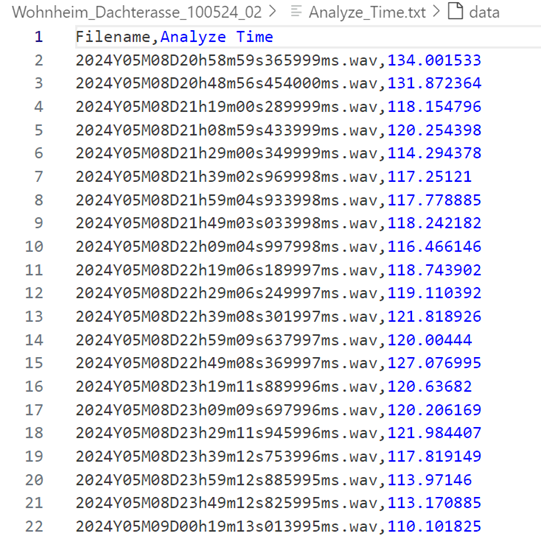
\includegraphics[width=1\linewidth]{bilder/analyze_time_wohnheim.png}
    \caption{Analysezeit des testversuch Nr. 1.1 / Wohnheim Dachterrasse mit overlap von 0}
    \label{fig:enter-label}
\end{figure}

%! da erst nach zwei Audiofiles analysiert wird, sind in den ersten beiden Spalten die files vertauscht. am besten händisch lösen
Die Analysezeit ist hier sogar länger als die Dauer der Audioaufnahme selbst.
Insgesamt hat die Session ... Sekunden gedaurt.

\subsubsection{Testversuch 1.2}

%python3 main110524.py --region COUNTRIES/Deutschland/Heiligenhaus/Wohnheim_Dachterasse_110524.py/ --rtype table --rtype2 audacity --coordinates True --hour 4 --minute 0 --lat 6.968352784 --lon 51.327644614 --trim 10:00 --overlap 1 --min_conf 0.3

Eckdaten:
Datum: 11.~05.~24
%Ordner: COUNTRIES/Deutschland/Heiligenhaus/Wohnheim_Dachterasse_110524
Dauer: 4h 
Koordinaten: True
Dauer pro Audio: 10 Minuten
Overlap: 0
Mindestwahrscheinlichkeit: 0.3


\begin{table}[]
\centering
\caption{Testversuch 1.2}
\label{tab:testversuch1_2}
\begin{tabular}{ll}
Datum                     & 11.05.24                                                                                                                           \\
Ordner                    & \begin{tabular}[c]{@{}l@{}}COUNTRIES/Deutschland/Heiligenhaus/\\ Wohnheim\_Dachterrasse\_110524\end{tabular}                       \\
Dauer                     & 4 h                                                                                                                                \\
Koordinaten               & \begin{tabular}[c]{@{}l@{}}--lon: 51.327644614\\ --lat: 6.96835278\\ --coordinates True\\ Koordinaten wurden gefunden\end{tabular} \\
Dauer pro Audio           & 10:00                                                                                                                              \\
Overlap                   & 0 (default)                                                                                                                        \\
Mindestwahrscheinlichkeit & 0.1 (default)                                                                                                                     
\end{tabular}
\end{table}



\begin{table}[]
\centering
\caption{Testversuch 1.2}
\label{tab:testversuch1_2}
\begin{tabular}{ll}
Datum                     & 11.05.24      \\
Ordner      & \begin{tabular}[c]{@{}l@{}}COUNTRIES/Deutschland/Heiligenhaus/\\ Wohnheim\_Dachterrasse\_110524\end{tabular}                       \\
Dauer                     & 4,0 Stunden\\
Koordinaten & \begin{tabular}[c]{@{}l@{}}--lon: 51.327644614\\ --lat: 6.96835278\\ --coordinates True\\ Koordinaten wurden gefunden\end{tabular} \\
Dauer pro Audio           & 10:00         \\
Overlap                   & 0 (default)   \\
Mindestwahrscheinlichkeit & 0.1 (default)
\end{tabular}
\end{table}


\begin{table}[]
\centering
\caption{Testversuch 1.2}
\label{tab:testversuch1_2}
\begin{tabular}{|l|l|}
\hline
Datum                     & 11.05.24      \\ \hline
Ordner      & \begin{tabular}[c]{@{}l@{}}COUNTRIES/Deutschland/Heiligenhaus/\\ Wohnheim\_Dachterrasse\_110524\end{tabular}                       \\ \hline
Dauer                     & 4,0 Stunden\\ \hline
Koordinaten & \begin{tabular}[c]{@{}l@{}}--lon: 51.327644614\\ --lat: 6.96835278\\ --coordinates True\\ Koordinaten wurden gefunden\end{tabular} \\ \hline
Dauer pro Audio           & 10:00         \\ \hline
Overlap                   & 0 (default)   \\ \hline
Mindestwahrscheinlichkeit & 0.1 (default) \\ \hline
\end{tabular}
\end{table}


\subsubsection{Ergebnisse der Analysezeit}
\begin{figure}
    \centering
    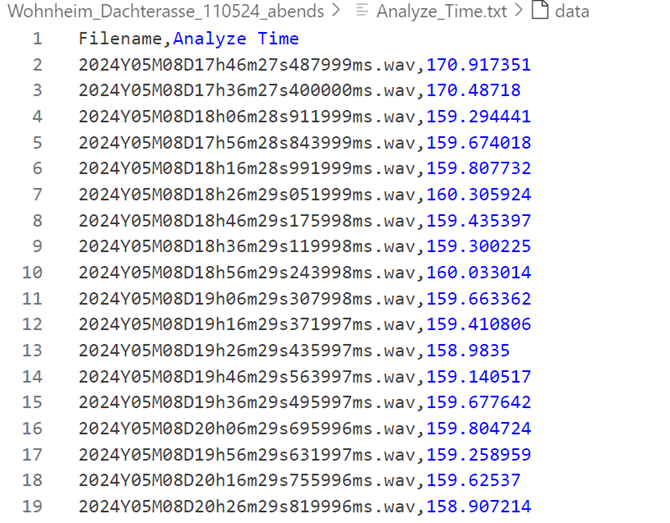
\includegraphics[width=1\linewidth]{bilder/analyze_time_wohnheim_02.png}
    \caption{Enter Caption}
    \label{fig:enter-label}
\end{figure}

\subsubsection{Validierung}


\begin{table}[]
\centering
\caption{11.$\sim$05.$\sim$2024 08:30 Uhr - 8:40 Uhr}
\label{tab:2024Y05M09D08h30m28s201983ms}
\begin{tabular}{|l|l|l|l|l|l|l|}
\hline
Zeitintervall in Sek & Zeitintervall in mm:ss & BirdNET Vogelart & Confidence & Merlin ID & Ohr (0; 0.5; 1) & Klassifikation \\ \hline
63.0  & 01:03 & Tree Pipit        & 0.6763 & -                 & 1 & :| \\ \hline
447.0 & 07:27 & Common Swift      & 0.9929 & -                 & 1 & :| \\ \hline
465.0 & 07:45 & Common Swift      & 0.7170 & European Robin    & 1 & :| \\ \hline
474.0 & 07:54 & Common Chiffchaff & 0.7823 & Common Chiffchaff & 1 & :) \\ \hline
498.0 & 08:18 & Common Chiffchaff & 0.6213 & Common Chiffchaff & 1 & :) \\ \hline
507.0 & 08:27 & Common Chiffchaff & 0.5170 & Common Chiffchaff & 1 & :) \\ \hline
525.0 & 08:45 & Common Chiffchaff & 0.8636 & Common Chiffchaff & 1 & :) \\ \hline
537.0 & 08:57 & Common Chiffchaff & 0.8070 & Common Chiffchaff & 1 & :) \\ \hline
\end{tabular}
\end{table}




\subsection{Testversuch 2  - Balkon in Unterilp}


%Beschreibung des Versuchsaufbau:
Abdeckung zum Schutz vor Wärmeeinstrahlung
Mikrofon hängt über Geländer, um möglichst ohne Schallwände drumherum die Umgebung klar aufnehmen zu können
\begin{figure}
    \centering
    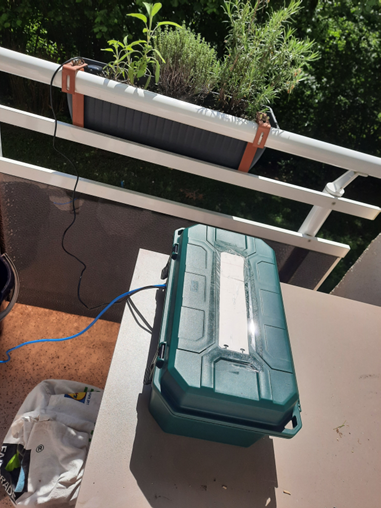
\includegraphics[width=1\linewidth]{bilder/balkon_01.png}
    \caption{Ablageort der Box: Tisch auf dem Balkon}
    \label{fig:enter-label}
\end{figure}

\begin{figure}
    \centering
    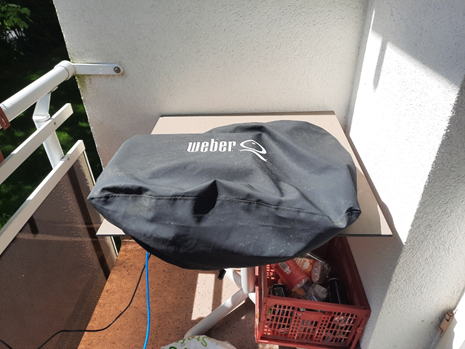
\includegraphics[width=1\linewidth]{bilder/balkon_02.png}
    \caption{Plane als Sonnenschutz über die Box gelegt}
    \label{fig:enter-label}
\end{figure}

\begin{figure}
    \centering
    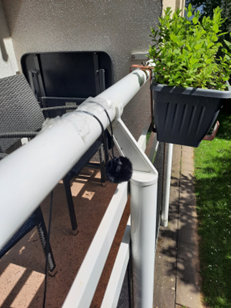
\includegraphics[width=1\linewidth]{bilder/balkon_03.png}
    \caption{Mikrofon hängt über das Balkongeländer, ist mit Tesafilm am Kabel fixiert}
    \label{fig:enter-label}
\end{figure}

\begin{figure}
    \centering
    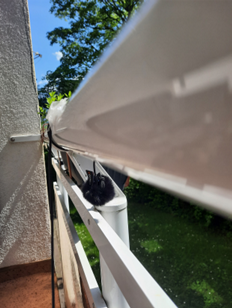
\includegraphics[width=1\linewidth]{bilder/balkon_04.png}
    \caption{weiteres Bild vom Mirkofon aus einem anderen Blickwinkel}
    \label{fig:enter-label}
\end{figure}


\subsubsection{Ergebnisse der Analysezeit}


\begin{figure}
    \centering
    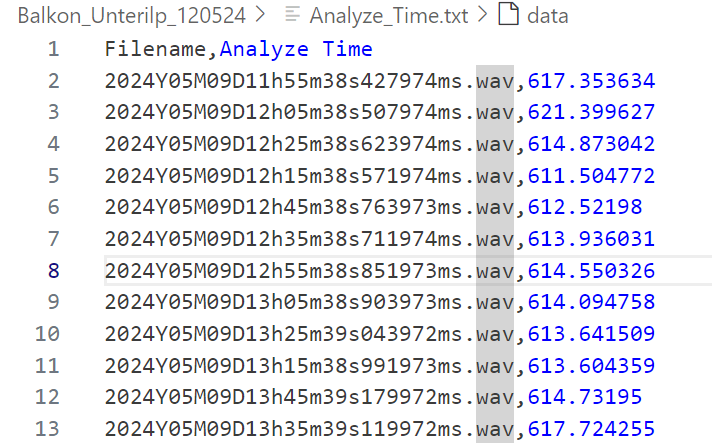
\includegraphics[width=1\linewidth]{bilder/analyze_time_balkon.png}
    \caption{Analysezeit des Testversuch Nr. 2 / Balkon Unterilp mit einem overlap von 2.5}
    \label{fig:analyze_time_balkon}
\end{figure}


\subsection{Start der Software}

-> Vorbereitung z.B. species-list anlegen
-> Verbindung mit dem Jetson aufbauen
-> Befehl an den Jetson schicken


\subsection{}

vierundzwanzig Stunden später:

Was sind die Ergebnisse?



